%%%%%%%%%%%%%%%%%%%%%%%%%%%%%%%%%%%%%%%%%
% Beamer Presentation
% LaTeX Template
% Version 1.0 (10/11/12)
%
% This template has been downloaded from:
% http://www.LaTeXTemplates.com
%
% License:
% CC BY-NC-SA 3.0 (http://creativecommons.org/licenses/by-nc-sa/3.0/)
%
%%%%%%%%%%%%%%%%%%%%%%%%%%%%%%%%%%%%%%%%%

%----------------------------------------------------------------------------------------
%	PACKAGES AND THEMES

\documentclass{beamer}

\mode<presentation> {

% The Beamer class comes with a number of default slide themes
% which change the colors and layouts of slides. Below this is a list
% of all the themes, uncomment each in turn to see what they look like.

%\usetheme{default}
%\usetheme{AnnArbor}
%\usetheme{Antibes}
%\usetheme{Bergen}
%\usetheme{Berkeley}
%\usetheme{Berlin}
%\usetheme{Boadilla}
%\usetheme{CambridgeUS}
\usetheme{Copenhagen}
%\usetheme{Darmstadt}
%\usetheme{Dresden}
%\usetheme{Frankfurt}
%\usetheme{Goettingen}
%\usetheme{Hannover}
%\usetheme{Ilmenau}
%\usetheme{JuanLesPins}
%\usetheme{Luebeck}
%\usetheme{Madrid}
%\usetheme{Malmoe}
%\usetheme{Marburg}
%\usetheme{Montpellier}
%\usetheme{PaloAlto}
%\usetheme{Pittsburgh}
%\usetheme{Rochester}
%\usetheme{Singapore}
%\usetheme{Szeged}
%\usetheme{Warsaw}

% As well as themes, the Beamer class has a number of color themes
% for any slide theme. Uncomment each of these in turn to see how it
% changes the colors of your current slide theme.

%\usecolortheme{albatross}
%\usecolortheme{beaver}
%\usecolortheme{beetle}
%\usecolortheme{crane}
%\usecolortheme{dolphin}
%\usecolortheme{dove}
%\usecolortheme{fly}
%\usecolortheme{lily}
%\usecolortheme{orchid}
%\usecolortheme{rose}
%\usecolortheme{seagull}
%\usecolortheme{seahorse}
%\usecolortheme{whale}
%\usecolortheme{wolverine}

%\setbeamertemplate{footline} % To remove the footer line in all slides uncomment this line
%\setbeamertemplate{footline}[page number] % To replace the footer line in all slides with a simple slide count uncomment this line

%\setbeamertemplate{navigation symbols}{} % To remove the navigation symbols from the bottom of all slides uncomment this line
}

\usepackage{listings}

\usepackage{graphicx} % Allows including images
\usepackage{amssymb}
\usepackage{algorithmic}
%\usepackage{booktabs} % Allows the use of \toprule, \midrule and \bottomrule in tables
\makeatletter
\newenvironment{algorithm}[1][]{%
  \def\@captype{algorithm}%
  \par\nobreak\begin{center}\nobreak}
  {\par\nobreak\end{center}\nobreak}
\newcounter{algorithm}
\renewcommand\thealgorithm{\@arabic\c@algorithm}
\makeatother
%----------------------------------------------------------------------------------------
%	TITLE PAGE
%----------------------------------------------------------------------------------------

\title{Optimization using Metaheuristics\\
University Timetabling} % The short title appears at the bottom of every slide, the full title is only on the title page


\author{Martin Wiboe, Burak Topal, Too Sheng Tack} % Your name


\institute[DTU] % Your institution as it will appear on the bottom of every slide, may be shorthand to save space
{

DTU 2015
 \\ % Your institution for the title page
\medskip

}
\date{\today} % Date, can be changed to a custom date

\begin{document}
	\definecolor{darkgreen}{RGB}{0,100,0}
	
	\defverbatim[colored]\lstI{
		\begin{lstlisting}[language=Java,basicstyle=\ttfamily,keywordstyle=\color{blue},commentstyle=\color{darkgreen}]
// Total no. of lectures for a course
int[] courseAssignmentCount

// No. of course lectures on each day
int[][] courseLecturesOnDay

// No. of distinct working days for a course
int[] courseWorkingDays
		\end{lstlisting}
	}
	
		\defverbatim[colored]\lstII{
			\begin{lstlisting}[language=Java,basicstyle=\ttfamily,keywordstyle=\color{blue},commentstyle=\color{darkgreen}]
// No. of lectures in room for each course
int[][] lecturesInRoomForCourse

// Is lecturer busy in given time slot?
boolean[][][] lecturerBusy

// Is curriculum assigned in given time slot?
boolean[][][] curriculumAssigned
			\end{lstlisting}
		}

\begin{frame}
\titlepage % Print the title page as the first slide
\end{frame}

\begin{frame}
\frametitle{Overview} % Table of contents slide, comment this block out to remove it
\tableofcontents 
\end{frame}

%----------------------------------------------------------------------------------------
%	PRESENTATION SLIDES
%----------------------------------------------------------------------------------------

%------------------------------------------------
\section{Introduction} 
%------------------------------------------------


\begin{frame}
\frametitle{Introduction}
Every semester universities face the problem of creating good feasible timetable due to many complex constraints that have to be taken into consideration.
\begin{itemize}
\item Limited room capacity
\item A lecturer can teach more than one courses to be scheduled in different time slots
\item A curriculum has more than one courses to be scheduled in different time slots
\item Also lecturers and students have preferences
\end{itemize}
\end{frame}
%------------------------------------------------
\section{Metaheuristic} 
\begin{frame}
\frametitle{Metaheuristics}
A high level procedure to find a solution for given optimization problem.
\begin{itemize}
\item Efficient and practical 
\item Do not guarantee an optimal solution
\end{itemize}
Different types of metaheuristics:
\begin{itemize}
\item Hill Climber
\item Simulated Annealing
\item TABU
\end{itemize}
\end{frame}

%------------------------------------------------


\begin{frame}
	\frametitle{Neighborhood Function}
	The neighbors are the set of different "\textit{adjacent}" solutions.
	
	Neighbors of a solution $S$ are all solutions that can be reached by applying one of these functions to $S$:
	\begin{itemize}
		\item \textbf{add} a lecture to the schedule by filling an empty room
		\item \textbf{remove} a lecture that is currently scheduled, leaving an empty room
		\item \textbf{swap} two scheduled lectures
	\end{itemize}
\end{frame}

%------------------------------------------------

\section{Delta Evaluation}
\begin{frame}
	\frametitle{Evaluating the Schedule}
	To determine value of a schedule, our na{\"i}ve solution considers all:
	\begin{itemize}
		\item time slots
		\item rooms
		\item courses
		\item curricula
	\end{itemize}
	
	Time complexity is $\mathcal{O}(|T||R| + |T||C| + |T||Q|)$
\end{frame}

\begin{frame}
	\frametitle{Delta Evaluation}
	Extra bookkeeping to increase evaluation speed of modified solution.
	
	Trade memory and complexity for better performance.
	
	\begin{block}{Insights}
		\begin{itemize}
			\item \emph{add} and \emph{remove} only affects the given course $+$ neighbors.
			\item \emph{swap} is equal to \{\emph{remove}, \emph{remove}, \emph{add}, \emph{add}\}
		\end{itemize}	
	\end{block}
	
\end{frame}

\begin{frame}
	\frametitle{Bookkeeping}
	\lstI
\end{frame}

\begin{frame}
	\frametitle{Bookkeeping cont.}
	\lstII
\end{frame}

\begin{frame}
	\frametitle{Delta Evaluation is Significantly Faster}
	After optimizations:
	
	\begin{itemize}
		\item evaluate a neighbor solution in $\mathcal{O}(q)$
		\item update the bookkeeping state in $\mathcal{O}(q)$
	\end{itemize}
	
	$q$ is number of curricula for affected course, typically few. Can be further reduced to $\mathcal{O}(1)$.
	
	Overall speedup in our tests was more than 200x, depending on the data set.
\end{frame}

%------------------------------------------------

\begin{frame}
\frametitle{Hill Climber}
Incremental local search algorithm. 
\begin{itemize}
\item Easy to implement
\item Traps in local optimum
\end{itemize}
\begin{algorithm}[H]
\begin{algorithmic}[1]
\STATE {$select\;inital\;solution\;s_{0}$}
\STATE {$s^{*}=s_{0}$}
\REPEAT
\STATE {$select\;s\;\in N(s^{*})$}
\IF {$f(s) > f(s^{*})$}
\STATE {$ s^{*} = s$}
\ENDIF
\UNTIL {$time\;limit\;reached$}
\STATE{$\textbf{return}\;s^{*}$}
\end{algorithmic}
\caption{Hill Climber }
\label{alg:seq}
\end{algorithm}
\end{frame}

\begin{frame}
\frametitle{Hill Climber - Implementation Details}
Stochastic Hill Climber
\begin{itemize}
\item Fast average number of \textbf{??} iteration per seconds
\item Traps local optimum 
\item Different results for every run
\item Traps in local optimum
\end{itemize}
For each iteration selects the best state from two candidate Neighbours
\begin{itemize}
\item candidate state by removing a course in given time slot
\item candidate state by adding given  course in given time slot
\end{itemize}
\end{frame}

\begin{frame}[shrink=20]
\frametitle {Simulated Annealing}
Probabilistic optimization methods that uses the idea of the annealing process in thermodynamic.
\begin{itemize}
\item In high temperatures algorithm generally select the proposed action even it worse than the current solution.
\item Decreases the temperature for each iteration with given parameter
\end{itemize}

\begin{algorithm}[H]
\begin{algorithmic}[1]
\STATE {$select\;inital\;solution\;s_{0}$}
\STATE {$T=T_{start}$}
\STATE {$s^{*}=s_{0}$}
\REPEAT
\STATE {$select\;s\;\in N(s^{*})$}
\STATE {$\delta = f(s)- f(s^{*})$}
\IF {$\delta<0 or with probablity p(\delta,t_{i}$}
\STATE {$ s^{*} = s$}
\ENDIF
\STATE{$t_{i+1} = t_{i}*\alpha$}
\UNTIL {$time\;limit\;reached$}
\STATE{$\textbf{return}\;s^{*}$}
\end{algorithmic}
\caption{Simulated Annealing }
\label{alg:seq}
\end{algorithm}
\end{frame}

\begin{frame}[shrink=20]
\frametitle{Simulated Annealing  - Implementation Details}
Each iteration algorithm calculates the delta value with remove, assign and swap actions and chooses the best one. 
\begin{algorithm}[H]
\begin{algorithmic}[1]
\STATE {$\textbf{Search}(s_{0},T_{start},\alpha)$}
\STATE {$T=T_{start}$}
\STATE {$s^{*}=s_{0}$}
\REPEAT
\REPEAT
\STATE {$select\;day\;period\;room\;randomly$}
\STATE {$calculate;new\;solutions\;by\;assign\;remove\;abd\;swap\;operations$}
\UNTIL {$no\;hard\;constraint\;violations$}
\STATE {$selectbestaction\;m\in\lbrace Remove,Assign,Swap\rbrace\;has\;lowest\;f(s_{i}\oplus m) $}
\STATE {$\delta = f(s)- f(s_{i}\oplus m)$}
\IF {$\delta<0 or with probablity p(\delta,t_{i}$}
\STATE {$ s^{*} = s_{i}\oplus m$}
\ENDIF
\STATE{$t_{i+1} = t_{i}*\alpha$}
\UNTIL {$time\;limit\;reached$}
\STATE{$\textbf{return}\;s^{*}$}
\end{algorithmic}
\caption{Simulated Annealing - Pseudo Code}
\label{alg:seq}
\end{algorithm}
\end{frame}

\begin{frame}
\frametitle{TABU}
Uses local search paradigm and memory for optimization.
\begin{itemize}
\item Generally finds better solution than the other optimization problems
\item Contraction of the Tabu list is problem specific
\end{itemize}
\end{frame}

\begin{frame}
\frametitle{TABU - Neighbourhood Function Cont.}
Therefore for each iteration program generates;
\begin{itemize}
\item  $ d*p*r$ (max) number of neighbours by removing
\item  $d*(d-1)*p*(p-1)r*(r*1) $ (max) number of neighbours by swapping 
\item $ d*p*r*c$ (max) number of neighbours by by assigning
\item total max $d*(d-1)*p*(p-1)r*(r*1) + d*p*r $ and min $ d*p*r*c$ neighbours are generated in each iteration
\item d = number of days
\item p = number of periods per day
\item r = number of rooms
\item c = number of courses
\end{itemize}
\end{frame}

\begin{frame}[allowframebreaks] 
\frametitle{TABU  - Implementation Details}
\begin{algorithm}[H]
\begin{algorithmic}[1]
\STATE {$\textbf{Search}(s_{0},taboLength)$}
\STATE {$s^{*}=s_{0}$}
\REPEAT
\STATE {$ Calculate all neighbours of s and select the best one $}
\IF {$f(s_{neighbour})<f(s^{'}) and n=not in TABO List$}
\STATE {$  s^{'} = neighbour$}
\ENDIF
\STATE {$ s = s^{'}$}
\STATE {$ AddTaboList(action)$}
\IF {$f(s_{'})<f(s^{*})$}
\STATE {$ s^{*} = s^{'}$}
\ENDIF
\UNTIL {$time\;limit\;reached$}
\STATE{$\textbf{return}\;s^{*}$}
\end{algorithmic}
\caption{TABU - Pseudo Code}
\label{alg:seq}
\end{algorithm}
\end{frame}

\section{Results}
%------------------------------------------------

\begin{frame}
\frametitle{Parameter Tuning}
\begin{itemize}
\item 13 different test data, 15 runs for each test data
\item Simulated Annealing 
\begin{itemize}
\item 2 initial temperatures : 90 and 45
\item  3 cooling rate : 0.95, 	0.97,0.99
\end{itemize}
\item TABU: 
\begin{itemize}
\item 3 taboo length: 5, 10 and 20
\end{itemize}
\end{itemize}

\end{frame}

%------------------------------------------------
\begin{frame}
\frametitle{Simulated Annealing}
 \centerline{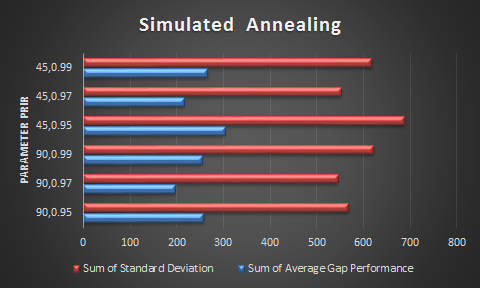
\includegraphics[width=1.0\textwidth]{simulated_annealing.png}}
\end{frame}
%------------------------------------------------
\begin{frame}
\frametitle{Simulated Annealing}
 \centerline{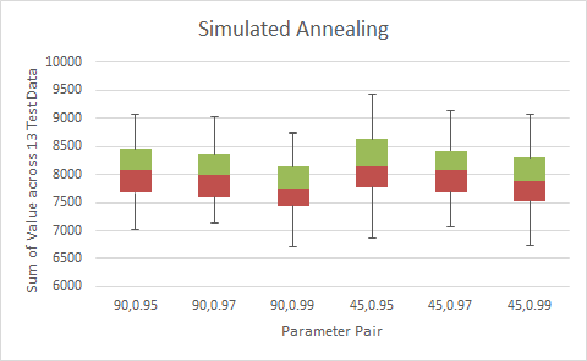
\includegraphics[width=1.0\textwidth]{simulated_annealing2.png}}
\end{frame}
%------------------------------------------------
\begin{frame}
\frametitle{TABU}
 \centerline{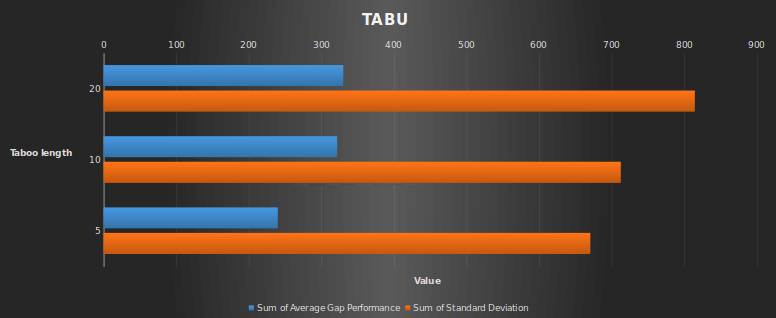
\includegraphics[width=0.8\textwidth]{TABU.png}}
\end{frame}
%------------------------------------------------
\begin{frame}
\frametitle{TABU}
 \centerline{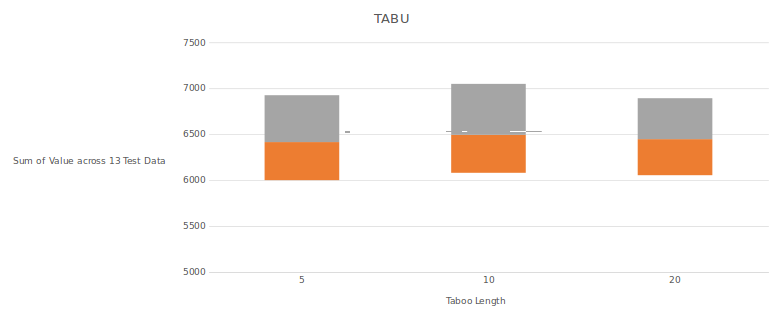
\includegraphics[width=1.0\textwidth]{TABU2.png}}
\end{frame}

\section{Conclusion}
%------------------------------------------------
\begin{frame}
\frametitle{Conclusion}

\begin{itemize}
	\item We used 3 different metaheuristics.
	
	\item Hill climber gets stuck in local optima.
	
	\item Simulated Annealing is very sensitive to parameters.
	
	\item TABU 5 gives consistently best results. Longer TABU lists are slower but might be warranted for larger problems.
\end{itemize}
\end{frame}


\begin{frame}
\Huge{\centerline{Questions?
		}}
\end{frame}

\end{document}
